
\section{Introduction}

\begin{frame}{}
  \begin{center}
    {\bf Part I: Introduction}
  \end{center}
\end{frame}

\subsection{Motivation}
\begin{frame}[t]{What is Computational Geometry?}
  In programming challenges, Computational Geometry problems involve answering questions about {\bf lines, points and angles}.

  \begin{block}{Example 1}
    Given a set of $N$ points $(s_1, s_2, s_3, \ldots, s_N)$, what is
    the area of the smallest polygon that covers all points in the set?
  \end{block}

  \centering
  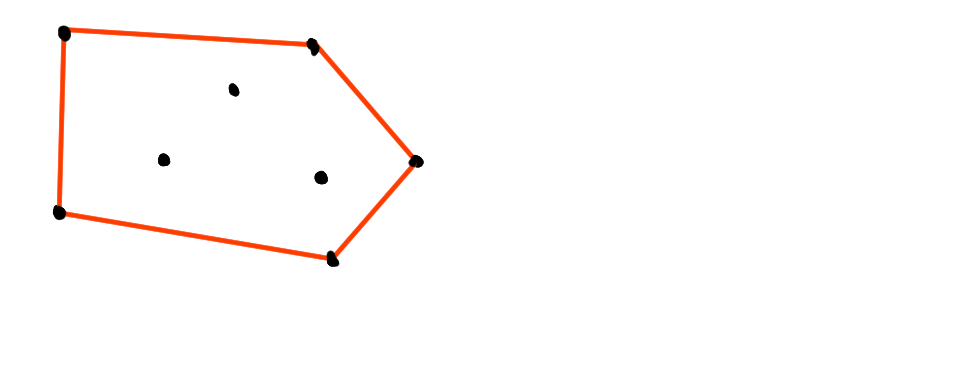
\includegraphics[width=0.8\textwidth]{img/sampleproblem_1.png}
\end{frame}

\begin{frame}[t]{What is Computational Geometry?}
  In programming challenges, Computational Geometry problems involve answering questions about {\bf lines, points and angles}.

  \begin{block}{Example 2}
    Given $N$ rectangles, $\{x_1,y_1,w_1,h_1\}; \ldots; \{x_N, y_N, w_N, h_N\}$, what is the smallest length of line segments needed to connect them?
  \end{block}

  \centering
  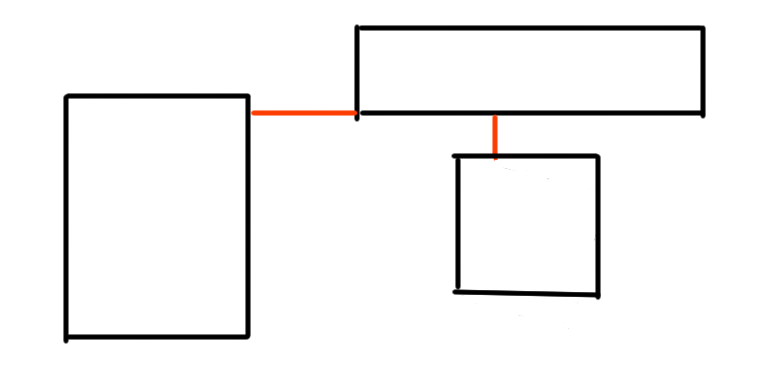
\includegraphics[width=0.5\textwidth]{img/sampleproblem_2.png}
\end{frame}

% TODO: Improve this image
\begin{frame}[t]{What is Computational Geometry?}
  In programming challenges, Computational Geometry problems involve answering questions about {\bf lines, points and angles}.

  \begin{block}{Example 3}
    Given a polygon and a set of $N$ points, find a line that divides the polygon in equal areas, with the same number of points in each area?
  \end{block}

  \begin{center}
    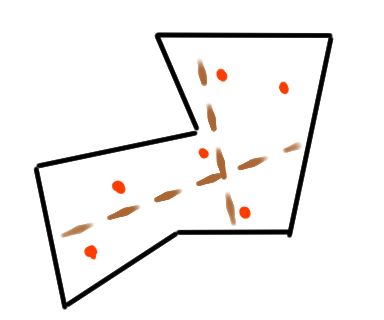
\includegraphics[width=0.3\textwidth]{img/sampleproblem_3.png}
  \end{center}
\end{frame}


\begin{frame}
  \frametitle{Computational Geometry: The good and the bad}

  \begin{block}{Positive Points}
    \begin{itemize}
      \item Geometry problems are fun, and you draw pretty pictures when thinking about them;
      \item A large part of geometry problems can be solved with algorithms and techniques that you learned in high school;
      \item The code for techniques is highly re-usable;
    \end{itemize}
  \end{block}

  \begin{alertblock}{Negative Points}
    \begin{itemize}
      \item You have to write a lot of code (but a lot of it is reusable!);
      \item Easy to get WE for small mistakes;
      \item Many special cases in the input data;
    \end{itemize}
  \end{alertblock}
\end{frame}


\begin{frame}
  \frametitle{Common Mistakes in Geometry Problems}

    \begin{block}{Errors because of special cases in input data}
      \begin{itemize}
        \item Multiple points in the same position;
        \item Collinear points (three points in the same line);
        \item Vertical lines (bad tangent value, division by 0);
        \item Parallel Lines (bad intersection value);
        \item Intersection at end of a segment;
        \item etc;
      \end{itemize}
    \end{block}

    \begin{block}{Floating Number Precision Errors}
      \begin{itemize}
        \item Wrong Answer because of poor rounding of final result;
        \item Error Propagation inside functions (multiplication, division);
      \end{itemize}
    \end{block}
\end{frame}


\begin{frame}[fragile]
  \frametitle{Common Mistakes in Geometry Problems}

  How to avoid these mistakes in Geometry Problems?\bigskip

  \begin{itemize}
    \item {\bf Special Cases}:
    \begin{itemize}
      \item Make sure to think which special cases affect your tecnique, and add checks for these cases;
      \item When testing your problem, include input with the special case;
    \end{itemize}\bigskip

    \item {\bf Precision Errors}:
    \begin{itemize}
      \item If possible, convert values to integers before calculation;
      \item When testing equality of two values, use an {\bf Epsilon Constant}:
\begin{verbatim}
if (float.1 == float.2) then            // NO
if (fabs(float.1 - float.2) < EPS) then // YES!
\end{verbatim}
    \end{itemize}
  \end{itemize}
\end{frame}

\subsection{Class Outline}
\begin{frame}
  \frametitle{Class Outline}
  In this lecture, we will focus on:
  \begin{itemize}
    \item Discussion of implementation of geometric operations;
    \item Discussion of problem examples;
  \end{itemize}\bigskip

  Specific topics will be:
  \begin{itemize}
    \item Intersection and Rotation of points and lines;\medskip
    \item Circle representation and components;\medskip
    \item Triangles (area, angles, triangles and circles);\medskip
    \item Polygon representation and Convex Hull;
  \end{itemize}\medskip
\end{frame}

\subsection{Problem Examples}

\begin{frame}
  \frametitle{Problem Example: Intersection}
    \begin{block}{}
      \begin{itemize}
      \item {\bf Input}: A rectangle and a line segment:
        \begin{itemize}
          \item Rectangle: $x_s y_s x_e y_e$
          \item Line: $x_0, y_0, x_1, y_1$
        \end{itemize}

      \item {\bf Output}\\
        {\bf True} if the line segment intersects the rectangle, {\bf False} if not
      \end{itemize}
    \end{block}
    \begin{columns}
      \column{.3\textwidth}
      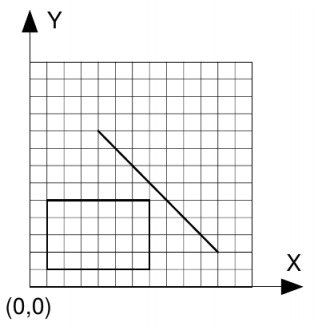
\includegraphics[width=.9\textwidth]{img/intersection_uva}
      \ppagenote{Problem image from \url{https://onlinejudge.org}}
      \column{.7\textwidth}
      How do you solve it?
    \end{columns}

\end{frame}

\begin{frame}[fragile]{Problem Example: Intersection}

  \begin{columns}
    \column{.35\textwidth}
    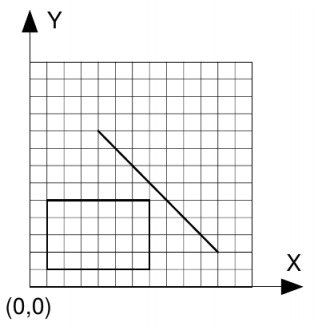
\includegraphics[width=\textwidth]{img/intersection_uva}
    \column{.65\textwidth}

    \begin{itemize}
      \item Test if $p_1$ or $p_2$ are inside the rectangle;
      \item For each segment $\overline{AB}$, test if $\overline{p_1,p_2}$ intersects $\overline{AB}$.\bigskip
{\smaller
\begin{verbatim}
int segmentIntersect(ax, ay, bx, by,
                     cx, cy, dx, dy)
{
  ta = (cx - dx)*(ay - cy) + (cy - dy)*(cx - ax);
  tb = (cx - dx)*(by - cy) + (cy - dy)*(cx - bx);
  tc = (ax - bx)*(cy - ay) + (ay - by)*(ax - cx);
  td = (ax - bx)*(dy - ay) + (ay - by)*(ax - dx);

  return tc*td <= 0 && ta*tb <= 0;
};
\end{verbatim}}
    \end{itemize}
  \end{columns}
\end{frame}

\begin{frame}
  \frametitle{Problem Example: Waterfalls}
    \begin{block}{}
      \begin{itemize}
      \item {\bf Input}
      \begin{itemize}
        \item List of line segments that block water;
        \item List of water sources;
      \end{itemize}

      \item {\bf Output}
      \begin{itemize}
        \item For every waterfall w, the end position $X_w$ where $Y_w=0$
      \end{itemize}
      \end{itemize}
    \end{block}

    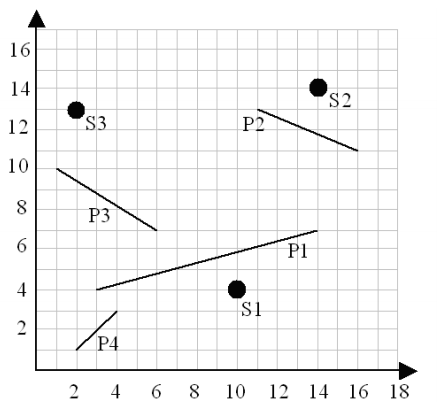
\includegraphics[width=0.30\textwidth]{img/waterfall}
    \ppagenote{Problem image from \url{https://onlinejudge.org}}
\end{frame}

\begin{frame}
  \frametitle{Problem Example: Waterfalls}
  \begin{columns}
    \column{0.4\textwidth}
      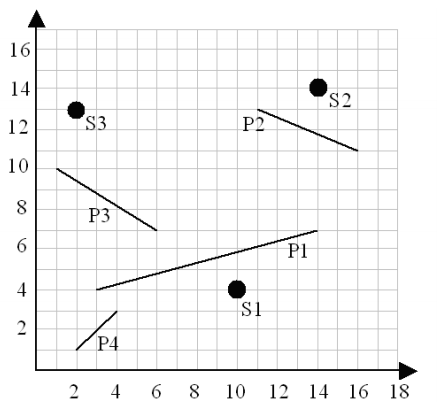
\includegraphics[width=1\textwidth]{img/waterfall}
    \column{0.6\textwidth}
    {\bf Full Search:}
    \begin{itemize}
      \item For each water source $S_i$:
      \begin{itemize}
        \item Calculate which segment intersects $\overline{S_i0}$ first.
        \item Adjust the position $X_i$ and repeat until $Y_i = 0$.
      \end{itemize}\bigskip

      \item This is a bit slow if there are many sources and segments.
      \item Can you pre-calculate something?
      \item Remember that all inputs are integers!
    \end{itemize}
  \end{columns}
\end{frame}
